\documentclass[a4paper,10pt]{scrartcl}
\usepackage[ngerman]{babel}
\usepackage[utf8x]{luainputenc}
\usepackage[headsepline,footsepline]{scrpage2}
\usepackage[autostyle=true,german=quotes]{csquotes}
\usepackage{graphicx}
\usepackage{eqlist}
\usepackage[left=25mm, right=25mm, top=27.5mm, bottom=40mm]{geometry}
\usepackage{calc}
\usepackage[justification=centering]{caption}
\usepackage{subcaption}
\usepackage{textcomp}
\usepackage{gensymb}
\usepackage[pdfa]{hyperref}
\usepackage{amsmath}
\usepackage{amsfonts}
\usepackage{amssymb}
\usepackage{tabularx}
\usepackage{multirow}
\usepackage{nicefrac}
\usepackage{float}

% \pdfminorversion=7
\usepackage{xmpincl}

\setlength{\headheight}{15mm}

\clearscrheadfoot
\lohead{
\includegraphics[height=1cm]{include/Logo_TU_Ilmenau.pdf}}
\cohead{Anleitung für den Linienscanner}
\rohead{Version \\ \parbox{\widthof{Version}}{\centering{1.0}}}
\lofoot{\vspace*{-3mm}TU Ilmenau, Fakultät MB, FG Qualitätssicherung und Industrielle Bildverarbeitung}
\cofoot{}
\rofoot{\vspace*{-3mm}\pagemark}
\pagestyle{scrheadings}

% opening
\title{Anleitung\\Linienscanner}
\author{\Large Benjamin Buch}
\date{\large \today}

\titlehead{
Technische Universität Ilmenau\\
Fakultät für Maschinenbau\\
Fachgebiet Qualitätssicherung und Industrielle Bildverarbeitung\\
Univ.-Prof. Dr. rer. nat. Gunther Notni
}

% Ausrichtung der description-Umgebung
\let\description=\eqlist
\let\enddescription=\endeqlist
\let\eqlistlabel\descriptionlabel

\renewcommand{\arraystretch}{1.5}

\begin{document}

\maketitle

\begin{center}
\begin{minipage}{0.6\textwidth}
\begin{description}
  \large
  \item[Autor $\ \ $] Benjamin Buch
  \item[Telefon] 03677~/~69~-~3975\\(Betreuer Dr.-Ing. Andreas Breitbarth)
  \item[E-Mail] benni.buch@gmail.com\\(andreas.breitbarth@tu-ilmenau.de)
\end{description}
\end{minipage}
\end{center}

\bigskip

\begin{abstract}
Der Linienscanner ist ein Messgerät zur 3D-Rekonstruktion. Der Arbeitsplatz
besteht aus dem Messgerät und einem PC mit Monitor, Maus und Tastatur. Das
Messgerät bestehend aus einem Linienlaser, einer 8-Bit-Grauwert-Kamera, sowie
einem XYZ-Verschiebetisch mit 2 Drehachsen, welche durch 2 MCL Boxen angesteuert
werden.
\end{abstract}

\bigskip

\begin{center}
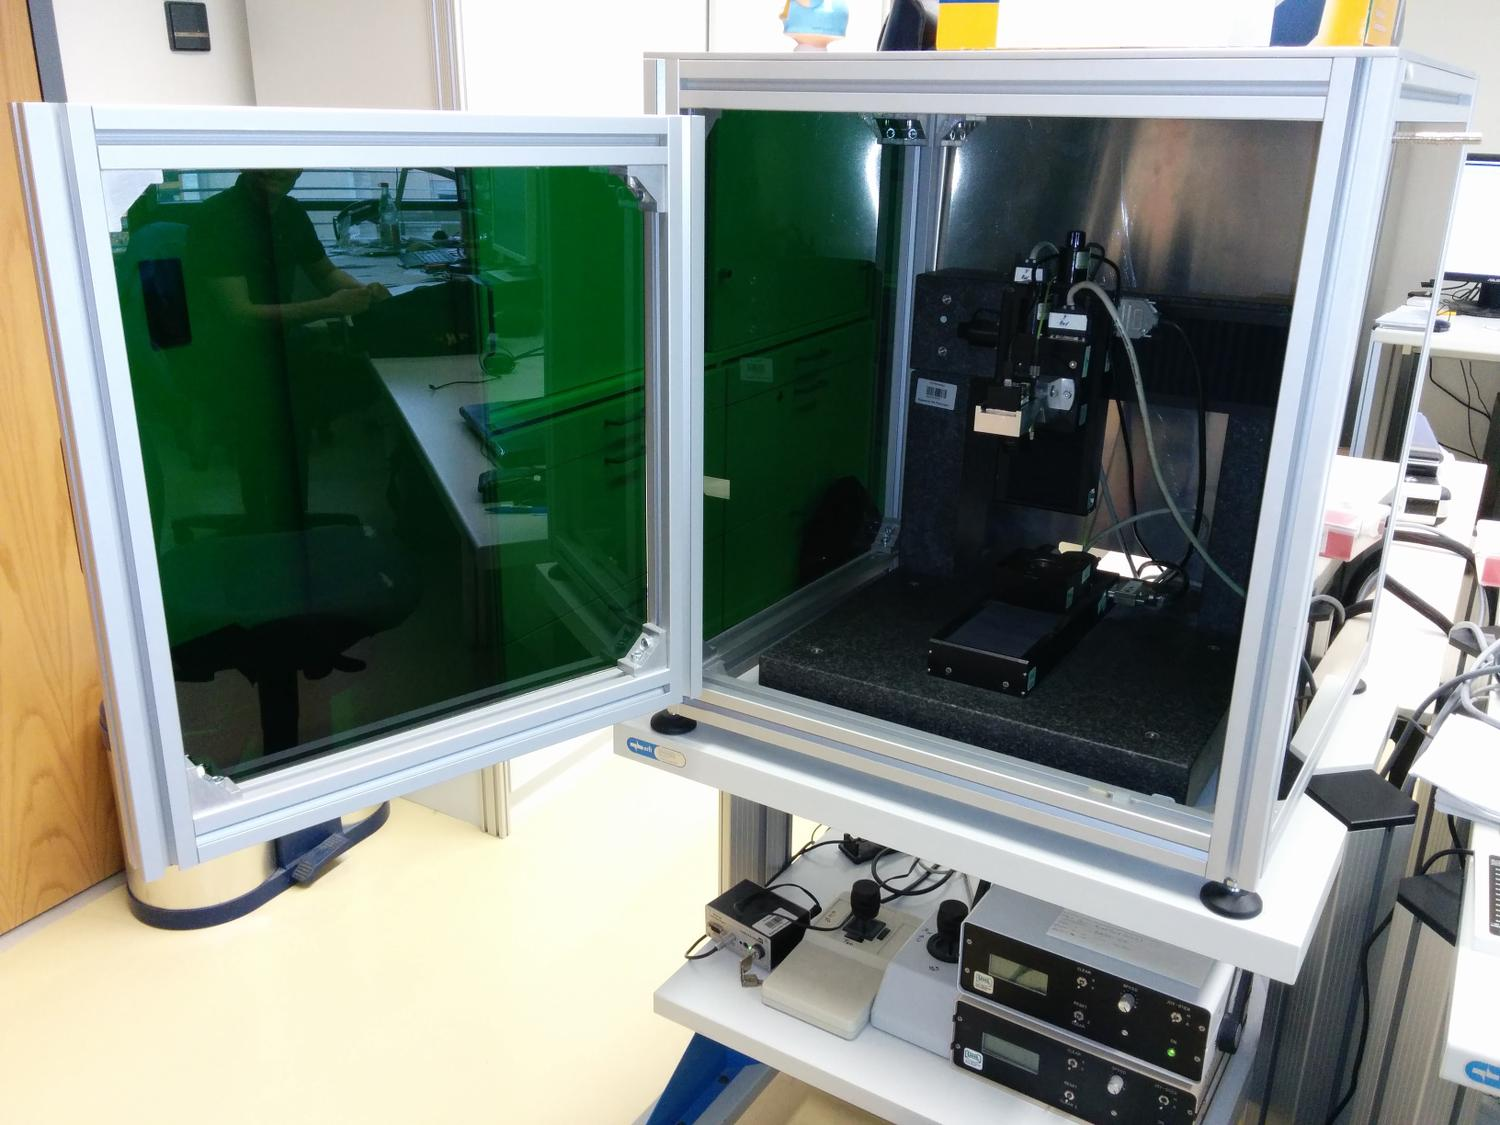
\includegraphics[width=0.7\textwidth]{include/IMG_20160412_140245.jpg}
\end{center}

\section{Begriffe und Definitionen}

Im vorliegenden Dokument werden 2D-Koordinaten mit Kleinbuchstaben (x, y) bezeichnet.
Für 3D-Koordinaten werden Großbuchstaben (X, Y, Z) verwendet.

\section{Einschalten}

Als Erstes sollte der PC eingeschaltet werden, da das Hochfahren aufgrund der alten Hardware
recht lange dauert. Das Login erfolgt über den Gast-Account.

Das Messgerät wird über einen Steckdosen-Verteiler, welcher sich hinter dem Gerät am Boden befindet
mit Strom versorgt. Ausgenommen hiervon ist die Kamera, welche ihren Strom per USB bezieht.

Für den Fall, dass Messgerät und PC noch nicht verbunden wurden, erfolgt nachfolgend die Beschreibung
des Anschließens. Mit dem PC verbunden sind nur die MCL-Boxen sowie die Kamera. Der Linienlaser kann
ausschließlich von Hand am Gerät bedient werden. Die untere MCL-Box steuert den Verschiebetisch in X, Y
und Z, die obere Box ist für die beiden Drehachsen verantwortlich. Zu beachten ist, dass die drehende
Box von der Software nicht angesteuert wird, sie muss also nicht angeschlossen werden.\footnote{
Die Drehachsen sind für den Messvorgang nicht notwendig und besitzen in Kalibrierrichtung keine
Endschalter, wodurch ihre Absolutposition nicht bestimmt werden kann. Daher wurden sie aus der
Messsoftware wieder entfernt.}

Von den MCL Boxen führt je ein Kabel mit serieller Schnittstelle zum PC. Um das Anschließen zu
vereinfachen, werden die Kabel auf einen 2-fach Serial-zu-USB-Adapter angesteckt. Ein weiteres
USB-Kabel führt von der Kamera zum PC. Der PC ist also letztlich über 2 USB-Kabel mit der Hardware
des Messgeräts verbunden.

Nachdem das System hochgefahren wurde und Sie sich im Gast-Account eingeloggt haben, muss das
Messprogramm »linescan« gestartet werden.

\section{Hardware}

\begin{figure}[h]
  \centering
  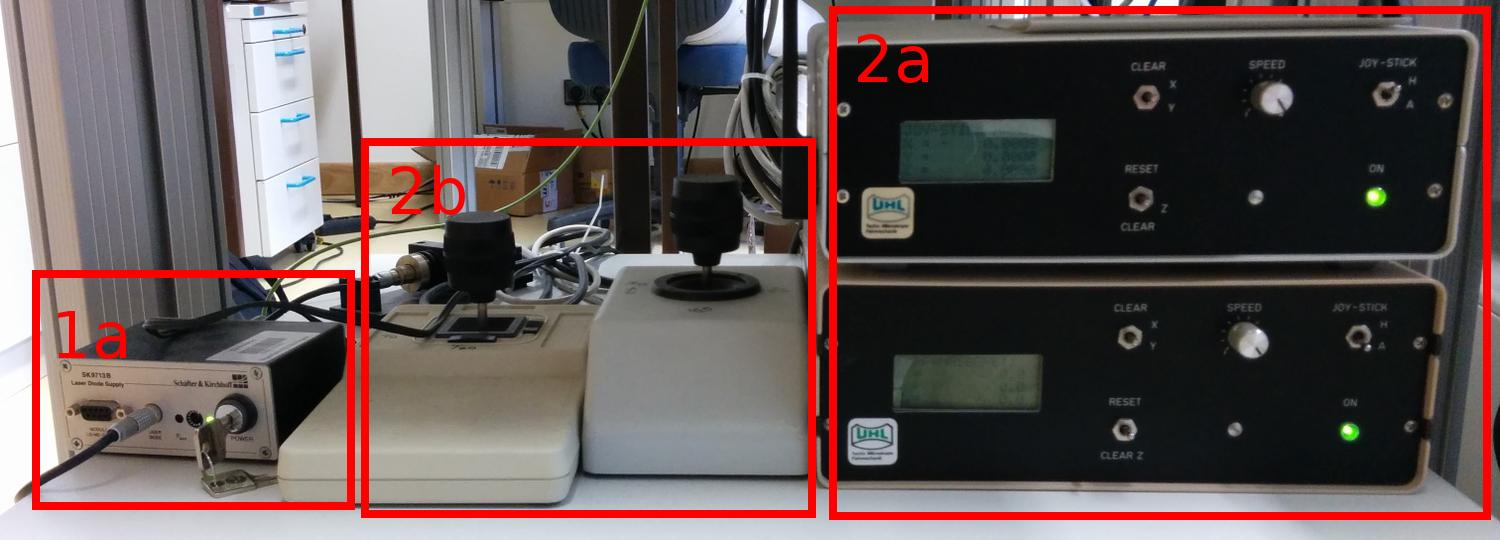
\includegraphics[width=\textwidth]{include/IMG_20160412_140339.jpg}
  \caption{Steuerhardware}
  \label{fig:overview}
\end{figure}

\begin{figure}[h]
  \centering
  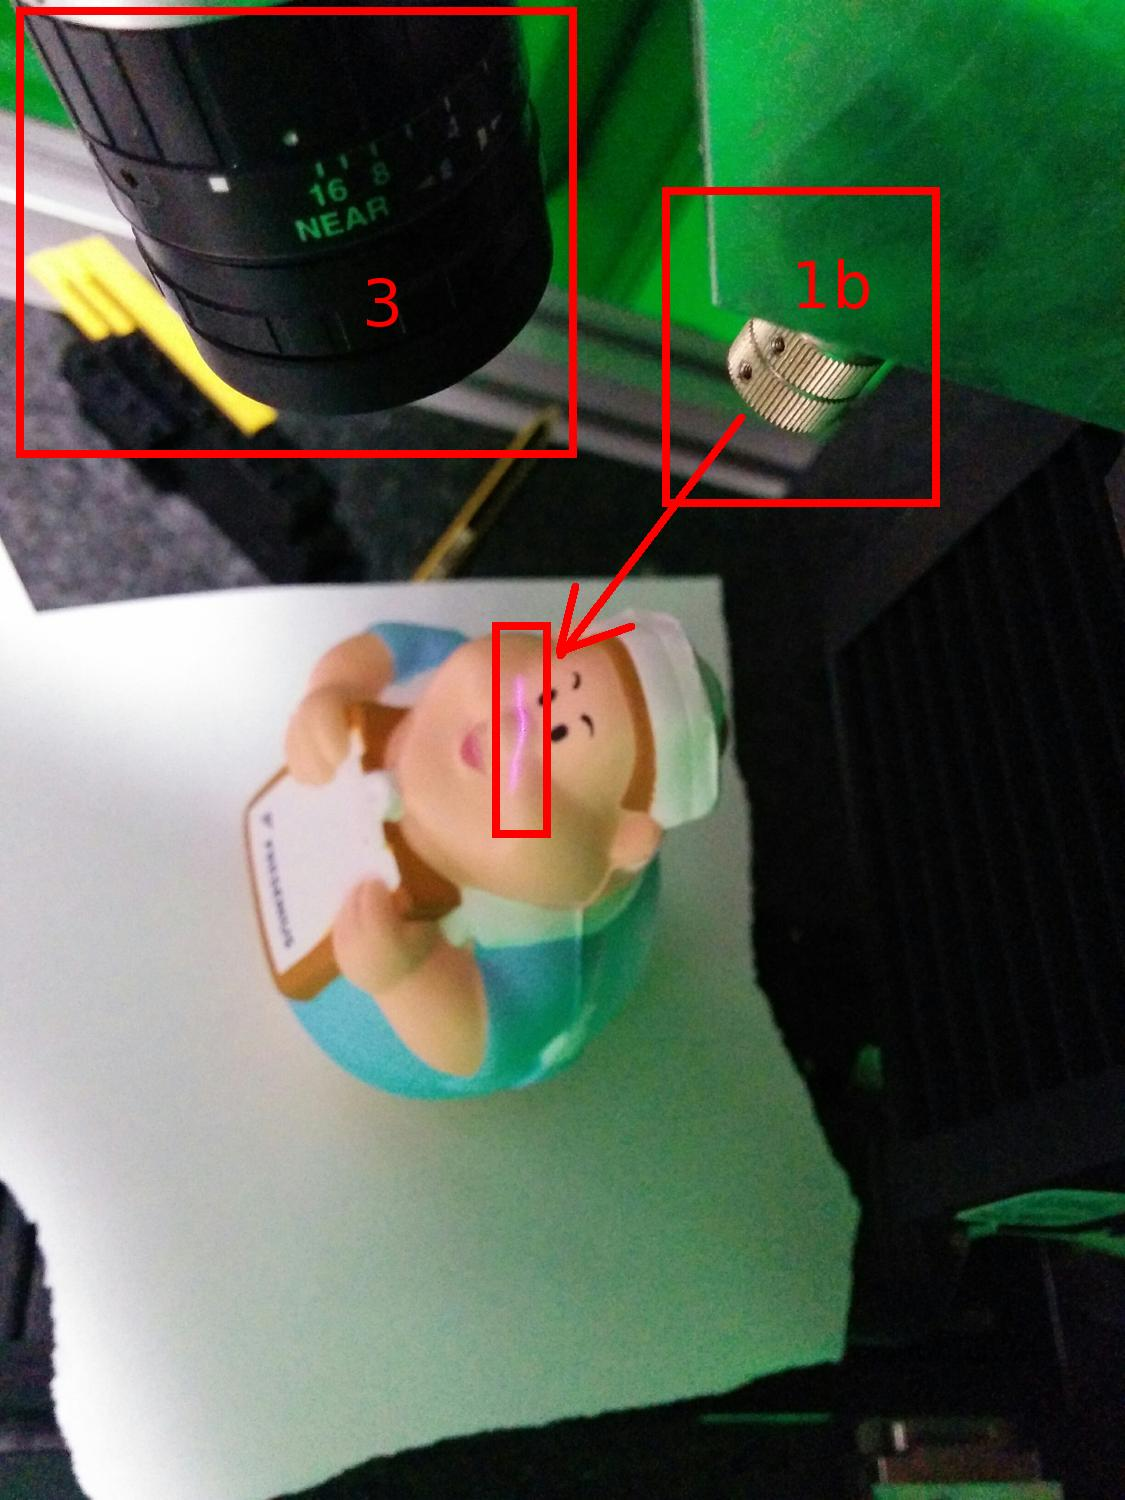
\includegraphics[width=0.5\textwidth]{include/IMG_20160412_135830.jpg}
  \caption{Hardware im Gehäuse}
  \label{fig:overview}
\end{figure}

\subsection{Linienlaser (1)}

Über die kleine Box mit dem Schlüssel (1a) kann der Linienlaser (1b) an- und ausgeschaltet werden.

\subsection{MCL Boxen (2)}

Die MCL-Boxen (2a) können wahlweise per PC (A-Stellung) oder per Joystick (2b, H-Stellung) gesteuert
werden. Will man die Z-Achse per Joystick steuert, muss man den Steuerknüppel drehen. Im Messbetrieb
ist immer die Steuerung per PC nötig.

\subsection{Kamera (3)}

Die Kamera wird ausschließlich von der Messsoftware am PC angesteuert.

\newpage

\section{Messsoftware}

\subsection{Kalibriermodus}

\begin{figure}[H]
  \centering
  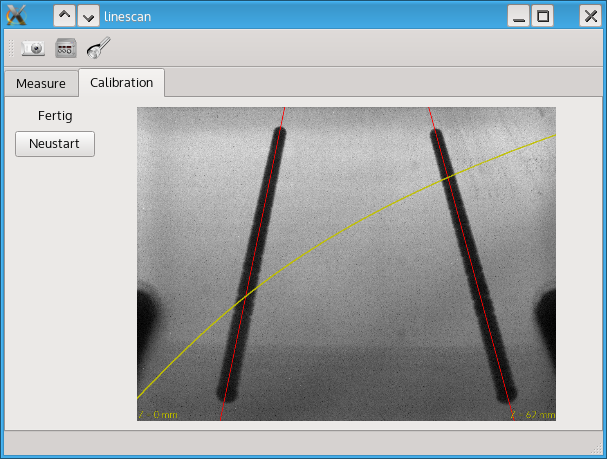
\includegraphics[width=0.5\textwidth]{include/calib.png}
  \caption{Ergebnis einer Kalibrierung}
  \label{fig:overview}
\end{figure}

Im Kalibriermodus erfolgt die Kalibrierung des Systems. Messungen können erst durchgeführt werden,
wenn eine gültige Kalibrierung existiert. Die Kalibrierung wird auf der Festplatte gespeichert.

\subsection{Messmodus}

\begin{figure}[H]
  \centering
  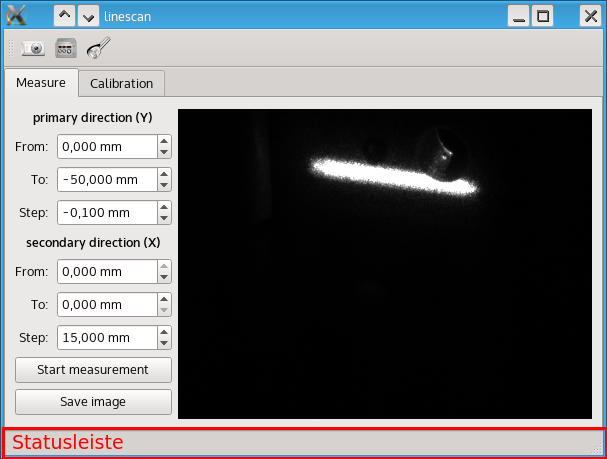
\includegraphics[width=0.5\textwidth]{include/measure.png}
  \caption{Messmodus}
  \label{fig:overview}
\end{figure}

Der Messmodus ist die Hauptkomponente des Programms. Dem Prinzip eines Linienscanners folgend,
wird für die Messung ein Bild mit der Laserlinie auf dem Messobjekt aufgenommen. Das Bild wird
in eine Liste von Punkten in der xy-Ebene der Kamera umgewandelt. Entsprechend der Kalibrierung
werden diese 2D-Punkte in 3D-Punkte transformiert und mit der aktuellen XYZ-Position des
Verschiebetisches (MCL) addiert. Anschließend fährt der Verschiebetisch an die nächste Position,
wo sich der Vorgang wiederholt.

Die Laserebene ist dabei identisch zur XZ-Ebene. Entsprechend erfolgt die Messung primär entlang
der Y-Achse. Um Objekte zu messen, welche breiter als die Laserlinie sind, kann die sekundäre
Richtung entlang der X-Achse erfolgen. Wurde das Messfeld in Y-Richtung komplett durchlaufen,
fährt der Tisch an die Y-Startposition und verschiebt das Objekt entsprechend der X-Richtung.
Dann wiederholt sich der Messvorgang in Y-Richtung.

Wurde das Messfeld komplett abgefahren, oder die Messung manuell unterbrochen, kehrt der Tisch
in die Startposition zurück und speichert das gemessene Objekt als ASCII-Punktwolke auf der
Festplatte. Der Dateiname wird für ein paar Sekunden in der Statusleiste des Programms angezeigt.

\subsection{MCL}

\begin{figure}[H]
  \centering
  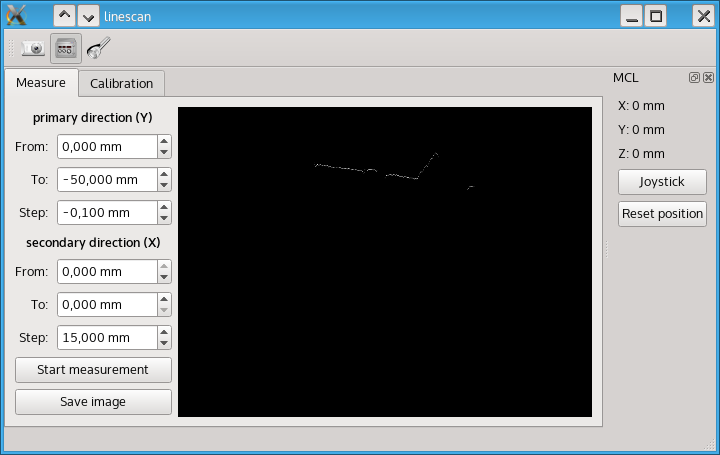
\includegraphics[width=0.5\textwidth]{include/mcl.png}
  \caption{MCL}
  \label{fig:overview}
\end{figure}

Das MCL-Dock kann über den entsprechenden Toolbar-Button ein- und ausgeblendet werden.
Hier werden die aktuellen Positionen des XYZ-Verschiebetisches angezeigt. Die Position kann
hier genullt werden. Außerdem kann die Joysticksteuerung softwareseitig aktiviert werden.

\textsl{Achtung:} Eine manuelle Umschaltung an der Box kann zu Inkonsistenzen führen, welche eine
falsche Skalierung der Messung zur Folge haben!

\subsection{Bildeinzug}

\begin{figure}[H]
  \centering
  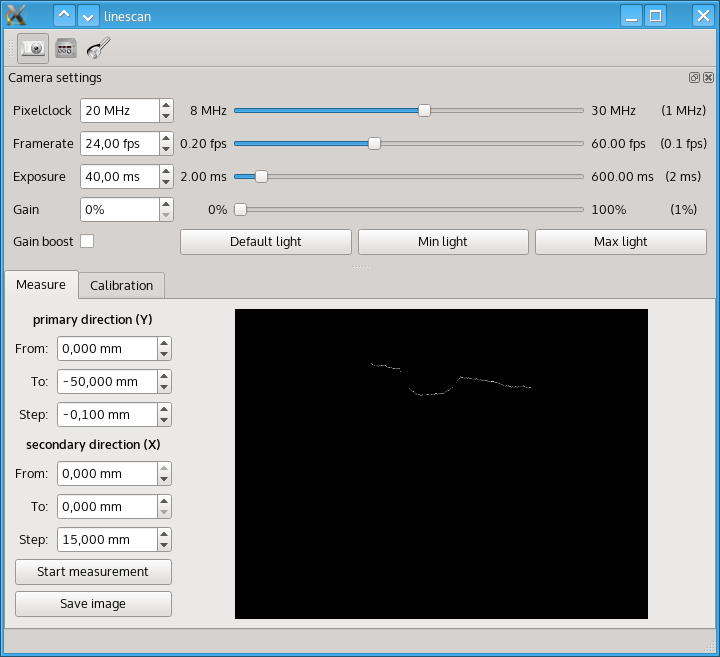
\includegraphics[width=0.5\textwidth]{include/cam.png}
  \caption{Bildeinzug}
  \label{fig:overview}
\end{figure}

Das Kamera-Dock kann über den entsprechenden Toolbar-Button ein- und ausgeblendet werden.
Hier sind alle Einstellungen zum Bildeinzug zu finden. Über die drei Buttons kann eine
Schnelleinstellung erfolgen.

\subsection{Linienberechnung}

\begin{figure}[H]
  \centering
  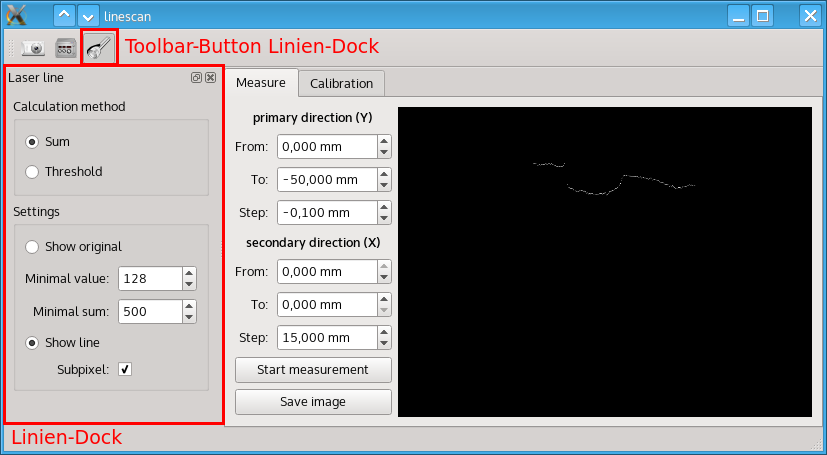
\includegraphics[width=0.5\textwidth]{include/laser.png}
  \caption{Linienberechnung}
  \label{fig:overview}
\end{figure}

Das Linien-Dock kann über den entsprechenden Toolbar-Button ein- und ausgeblendet werden.
Hier kann primär die Methode zur Detektion der Linie im Bild gewählt werden. Darunter kann
der gewählte Algorithmus parametriert werden. Zur besseren Veranschaulichung können die einzelnen
Schritte der Algorithmen durch Auswahl des entsprechenden Radio-Buttons dargestellt werden.

\section{Kalibrierung}

\begin{figure}[H]
  \centering
  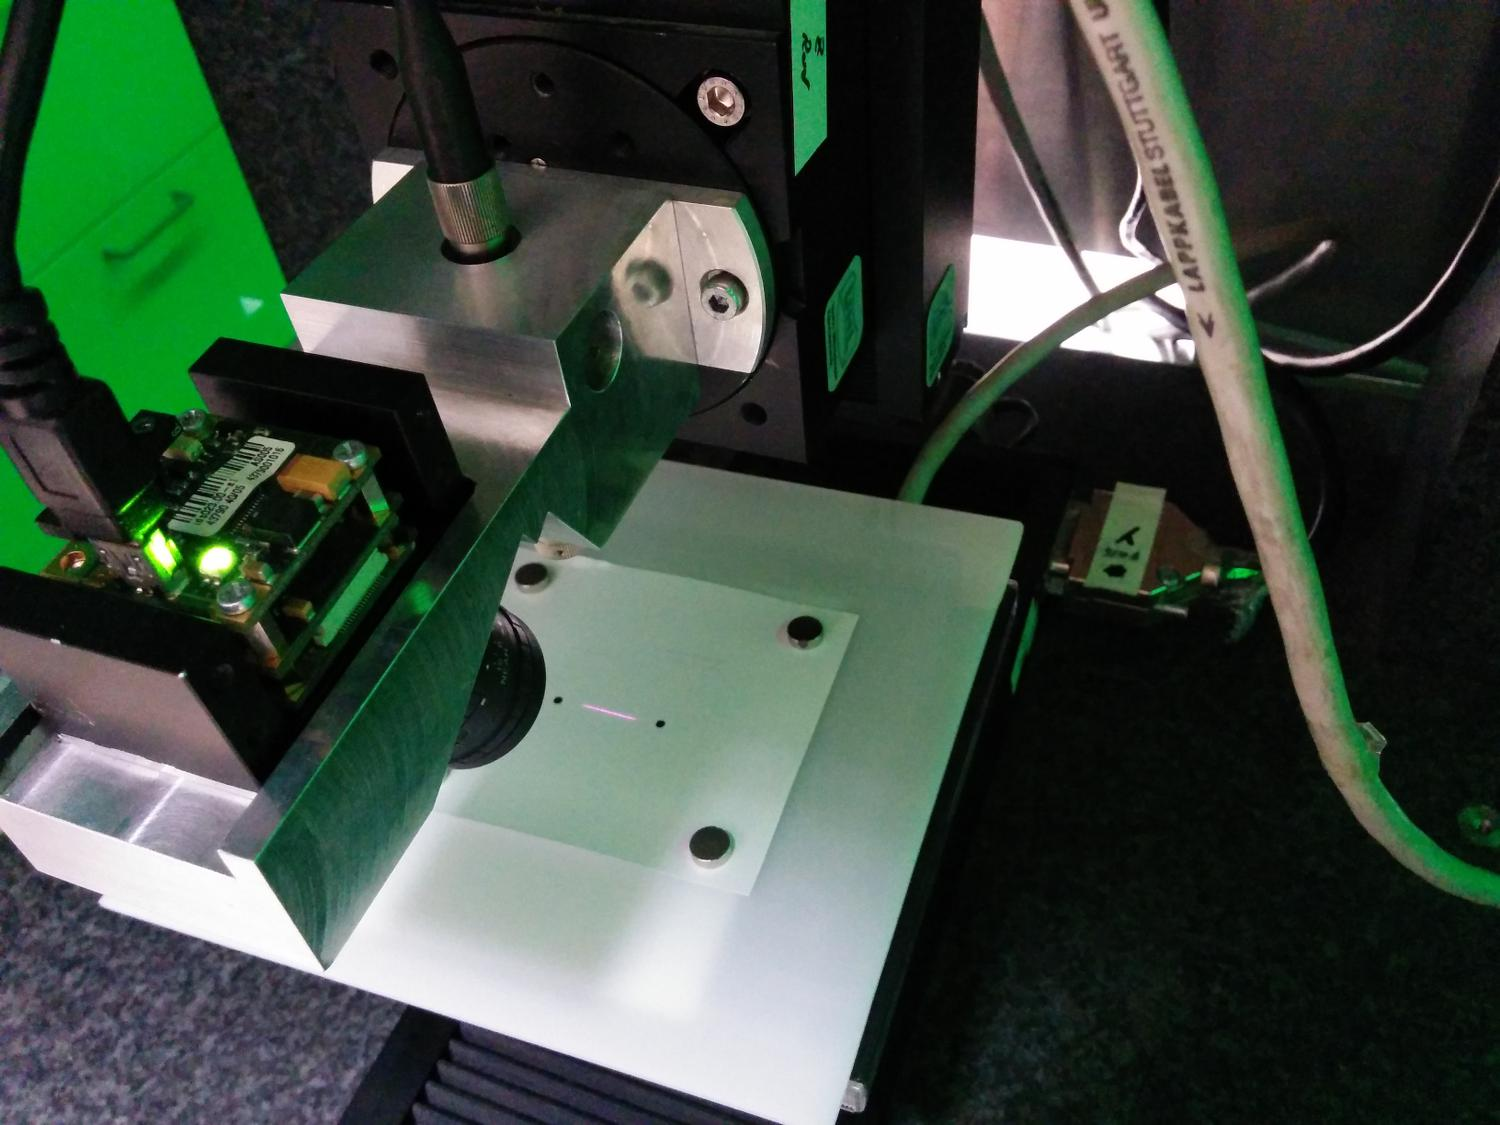
\includegraphics[width=0.5\textwidth]{include/IMG_20160412_162021.jpg}
  \caption{Kalibriertarget}
  \label{fig:overview}
\end{figure}

Die Kalibrierung erfolgt in drei Schritten.

Als Erstes wird das Kalibriertarget als Messobjekt eingelegt. Die Z-Achse muss nach ganz unten
gefahren werden. Dann wird der Linienlaser angeschaltet. Die Linie sollte zwischen den beiden
Kreisen liegen. Am PC wird die Linie erkannt und ihr Winkel berechnet. Mit dem Joystick für die
Drehachsen wird der Laser so ausgerichtet, dass die Linie einen Winkel von annähernd $0\degree$
hat. Dann wird der Button gedrückt.

Jetzt sucht das Programm nach den beiden Kreisen des Kalibriertargets. Dafür muss zunächst der
Linienlaser ausgeschaltet werden. Nun ist das Bild deutlich zu dunkel, daher wird im Kamera-Dock
die der Button für die maximale Helligkeit gedrückt. Die beiden Kreise müssen sich im unteren
Bildviertel befinden. Das Kalibriertarget muss von Hand so ausgerichtet werden, dass sich wiederum
ein Winkel von annähernd $0\degree$ ergibt. Auch dies ist durch einen Klick auf den Button zu
bestätigen.

Nun fährt der Verfahrtisch in Z-Richtung nach oben, bis die Kalibriertarget-Kreise vom oberen
Bildrand weniger weit entfernt sind, als sie es vom unteren waren. Für jede Position werden die
xy-Position der Kreismittelpunkte im Kamerabild sowie der Z-Koordinate des Verfahrtisches
aufgenommen.

Ist der Verfahrprozess abgeschlossen, erfolgt die Auswertung der aufgenommenen Daten. An die
Positionen der Target-Punkte wird jeweils eine lineare Funktion angefittet. Die linke Linie
wird als Nullposition im Objektkoordinatensystem definiert. Der Abstand der beiden Funktionen
ergibt die Umrechnung von Pixeln im mm anhand der y-Koordinate im Bild.

Da die Linien zwischen den beiden Kreisen nicht exakt $0\degree$ zur x-Richtung des Kamerabildes
haben, wird die y-Koordinate in der Bildmitte bzgl. der x-Richtung berechnet. Dann wird diese
y-Koordinate der Bilder, mit der aufgenommen Z-Koordinate des Verfahrtisches zu einer Menge von
Punkten kombiniert. An diese wird ein Polynom Dritten Gerades angefittet. Damit kann die
y-Koordinate des Bildes fortan direkt in die Z-Koordinate des Objektkoordinatensystems
überführt werden.

Als Kalibrierung ergibt sich somit:

\begin{flalign}
X &= X_\text{MCL} + \dfrac{x - left\_line(y)}{right\_line(y) - left\_line(y)} \cdot 25 mm\\
Y &= Y_\text{MCL}\\
Z &= Z_\text{MCL} + y\_to\_Z(y)
\end{flalign}

\end{document}
